\part{Praxisteil}

\section{Versuchsaufbau}
Der Optimierungsversuch kann leider nicht auf dem Livesystem durchgeführt werden, da dass die Stabilität beeinträchtigen würde. Deswegen wurde ein Entwicklungssystem genutzt, um die verschiedenen Methoden zu analysieren. Das Entwicklungssystem ist eine neuere Anschaffung der pludoni GmbH und dadurch, im Vergleich zum Livesystem, leistungsfähiger. Dadurch wird sich das Endergebnis, wenn es nach dem Abschluss der Arbeit auf das Livesystem übertragen wurde, in seinen Kenndaten unterscheiden. Trotz alledem werden die Verbesserungen relativ zum Testsystem proportional ausfallen. 

\begin{itemize}
 \item Testplattform: pludoni Server eq4
  \item Prozessor: Intel® Core™ i7-920 
  \item Arbeitsspeicher: 8 GB DDR3 RAM
  \item Festplatten: 2 x 750 GB SATA-II HDD (Software-RAID 1)
  \item Netzwerkverbindung: 100Mbit
  \item Server Software: Apache/2.2.16 (Module)
  \item PHP Version: PHP 5.2.6-1+lenny13 with Suhosin-Patch 0.9.6.2
  \item Mysql Version: 14.12 Distrib 5.0.51a 
  \item Betriebssystem: Debian 4.1.2-25 mit Kernel 2.6.26-26lenny2
  \item Serverstandort: Rechenzentrumspark Falkenstein
\end{itemize}

\section{Testverfahren}
Das Testen von Web-Performance hat sich in den letzten Jahren stetig weiterentwickelt. Eine Zeit lang galten sogenannte Backbonetests\footnote{Tests, die direkt am Backbone, also im Rechenzentrum durchgef\"uhrt werden. F\"uhrt zu besseren Ergebnissen, da der Client und der Testserver direkt verbunden sind. Dieser Test spiegelt aber nicht die Wirklichkeit wieder.} als das Non-Plus-Ultra. Nachdem aber immer deutlicher wurde, dass die tatsächlichen Ergebnisse sich stark von den Erwartungen unterscheiden, suchte man nach Alternativen. Der verlässlichste Test wird natürlich direkt beim Kunden beziehungsweise der Zielgruppe durchgeführt. Da es oft schwierig ist diese Tests durchzuführen, sollte zumindest mit ähnlichen Vorraussetzungen getestet werden.
\subsection{Servertest}
Die rein serverseitigen Optimierungen wurden mit "`ab"' getestet. "`ab"', das für "`apache bench"' steht, wurde entwickelt, um Apache Server zu testen. Es analysiert, wie lange ein Server braucht, um Webseiten auszuliefern und wieviele Anfragen er pro Sekunde befriedigen kann, ohne dass es zu Ausfällen kommt. "`ab"' führt die gewünschte Anzahl an Anfragen hintereinander, mit der gewählten Anzahl an nebenläufigen Zugriffen (Concurrency) auf die Ressource, aus und berechnet dann anhand der Ergebnisse die durchschnittliche Antwortzeit. Der Kommandozeilenbefehl, der zum Testen genutzt wurde, war denkbar einfach:
\begin{lstlisting}[language=bash,label="`ab"' mit Parametern,caption="`ab"' mit Parametern]
ab -n 50 -c 1 http://itsax.it-jobs-und-stellen.de/
\end{lstlisting}
Dies führt 50 Anfragen mit einer Concurrency von 1 auf itsax.it-jobs-und-stellen.de.

\subsection{Browsertest}
Browsertests k\"onnen durch die komplexen Voraussetzungen keine exakten Ergebnisse f\"ur alle m\"oglichen Konfigurationen liefern. Ein Netbook zum Beispiel wird eine Webseite immer langsamer darstellen als ein Desktop-PC der neuesten Generation. Man kann natürlich am eigenen Computer Tests durchführen. Dafür gibt es aber auch Programme, wie Firebug\footnote{Entwicklertool f\"ur Firefox \url{https://addons.mozilla.org/de/firefox/addon/firebug/}} und YSlow\footnote{Erweiterung f\"ur Firebug, die Webseiten bewerten kann. \url{https://addons.mozilla.org/de/firefox/addon/yslow/}}, die auch Verbesserungsvorschläge liefern können. Da aber möglichst objektiv getestet werden soll, ist es von Vorteil, eine standardisierte und automatisierte Umgebung zu nutzen. Für diesen Zweck bietet sich WebpageTest\footnote{Link: \url{https://sites.google.com/a/webpagetest.org/docs/}} an. Es wurde ursprünglich für den internen Gebrauch bei AOL entwickelt, steht aber seit 2008 unter der BSD-Lizenz und kann somit frei genutzt werden. Es ist eine umfassende Testsuite für Webseiten. Besonders die verschiedenen Analysen, die automatisch durchgeführt werden, sind positiv hervorzuheben. Das Programm ist in der Lage, die Webseite nach den "`Google Page Speed"'-Kriterien zu bewerten und ausführliche Inhaltsanalysen, aufgeschlüsselt nach Multipurpose Internet Mail Extensions(MIME)-Typen, zu liefern. Zusätzlich wird ein sehr hilfreiches Wasserfalldiagramm erzeugt und für jedes Element der Webseite ein Performance-Review erstellt. Darin werden unter anderem Kriterien wie Kompression und Caching betrachtet. Als besonderes Feature gibt es noch einen Videovergleich, in dem man Webseiten gegeneinander antreten lassen kann. Man kann WebpageTest sowohl selbst installieren als auch externe Anbieter nutzen. In diesem Fall wird www.webpagetest.org mit folgenden Parametern genutzt:
\begin{itemize}
  \item 10 konsekutive Tests
  \item Standort des Clients: Frankfurt a. M.a
  \item Browser: IE9
  \item Connection: DSL 1,5 Mbps / 50ms RTT
  \item Only First View\footnote{Nur ungecachte Zugriffe werden getestet.}
\end{itemize}
\subsection{Andere Analyseverfahren}
Profiling und Debugging auf Codeebene wurden nur sporadisch eingesetzt, da sie den Anwendungsfall Webseite nur eingeschränkt betreffen. Durch Caching kann die Codeausführungszeit größtenteils eliminiert werden. Bei Anwendungsfällen, die kein Caching erlauben, wie zum Beispiel eine Suche oder eine Applikation, ist es aber sehr hilfreich diese Tools zu verwenden. Sie ersparen viel Arbeit, da die Problemstellen schnell ausgemacht werden können. Von Hand diese Arbeiten durchzuführen, ist in kleinen Projekten sehr mühsam und in großen Projekten fast unmöglich. Jeder Entwickler sollte solche Programme in seinem Repertoire haben.
%TODO Brau
\section{Ausgangszustand}  
Sreeram Ramachandran, ein Software Ingenieur der Firma Google, hat eine Analyse über 4.2 Milliarden Seiten veröffentlicht. Diese ist im Rahmen der Initiative "`Let's make the web faster"' entstanden und zeigt häufige Fehlerquellen und ungenutztes Potential auf. Die durchschnittliche Webseite hat laut Ramachandran 320 kB Größe, 44 verschiedene Ressourcen und es werden nur 66\% der komprimierbaren Inhalte tatsächlich komprimiert.\citep{Google2011a}
ITsax.de hat 106 Ressourcen und 444 kB an Daten. Schon anhand dieser zwei Zahlen lässt sich eine vergleichsweise schwache Leistung vorhersehen. Besonders die Anzahl an verschiedenen Ressourcen deutet auf Missstände hin, da Parallelisierung von Zugriffen nur bis zu einem bestimmten Grad möglich ist. Die Time to First Byte(TtFB) von 674ms bezeichnet die Zeit, die vergeht bis der Webbrowser die ersten Daten empfängt. Der Nutzer hat aber zu diesem Zeitpunkt noch keinen Inhalt pr\"asentiert bekommen. Die Inhalte werden erst angezeigt, nachdem die Time to Start Render(TtSR) vergangen ist. Der Nutzer muss demnach ungefähr zwei Sekunden warten, bis die Webseite im Browser anfängt sich aufzubauen. Die Load Time(LT) bezeichnet dann die Zeit die vergeht, bis die Seite komplett dargestellt wird und der Benutzer sie ohne Einschränkungen bedienen kann. Es können aber auch nach der LT noch Inhalte nachgeladen werden, wie zum Beispiel gestreamte Videos oder andere asynchrone Inhalte. Diese nachgeladenen Inhalte wirken sich aber nicht mehr negativ auf die User Experience aus, solange sie im Rahmen bleiben und nicht wichtige Teile der Webseite, wie zum Beispiel das Hauptmenü, noch per Flash geladen werden müssen. Die Anzahl der DOM Elemente bezeichnet alle vom Browser zu verarbeitenden Objekte und ist ein Indikator für die Komplexität der Webseite. Je mehr Elemente also vorhanden sind, desto länger muss der Browser die Positionierung und Darstellung berechnen. Mit 855 DOM Elementen gehört ITsax.de leider schon zu den komplexeren Seiten, was zu einem Großteil Drupal anzurechnen ist, welches auf Kosten der Performance andere Aspekte, wie Konfigurierbarkeit, in den Vordergrund stellt. Die Inhalte auf der Seite Itsax.de wurden mit dem Analysetool webpagetest.org ausgewertet. Die Ergebnisse sind in Abbildung \ref{fig:startbyte} und \ref{fig:startrequest} dargestellt, einmal in Bezug auf Größe und einmal aufgeschlüsselt nach der Anzahl der benötigten Requests, um die Inhalte vom Server anzufordern. Die numerischen Werte sind in der Tabelle 1 respektive Tabelle 2 erfasst.
\begin{figure}[!ht]
  \centering
  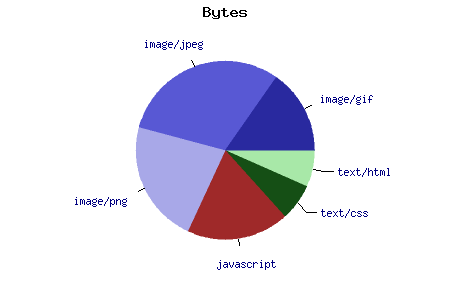
\includegraphics[scale=0.5]{material/start_byte_pie.png}
  \caption{Größe der Inhalte}
  \label{fig:startbyte}
\end{figure}
\begin{tabbing}
Request \quad\= blablabla \quad\= \kill
\textbf{Typ} 	 \> \textbf{Byte} \\
image/jpeg	\>142251\\
image/png	\>101428\\
javascript	\>84758\\
image/gif	\>73378\\
text/css	\>30222\\
text/html	\>29917\\
\end{tabbing}

\begin{figure}[!ht]
  \centering
  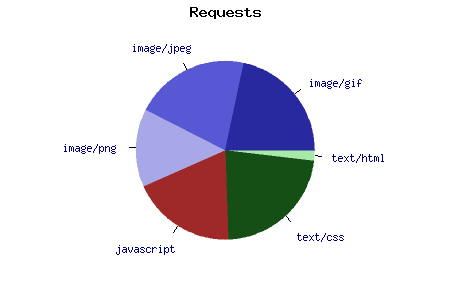
\includegraphics[scale=0.5]{material/start_request_pie.png}
  \caption{HTTP Anfragen}
  \label{fig:startrequest}
\end{figure}
\begin{tabbing}
Request \quad\= blablabla \quad\= \kill
\textbf{Typ} 	 \> \textbf{Anzahl} \\
text/css	 \>	24 	\\
image/gif	 \>	23 	\\
image/jpeg	 \>	22 	\\
javascript	 \>	20 	\\ 
image/png	 \>	15 	\\
text/html	 \>	2 	\\
\end{tabbing}
Leicht zu erkennen ist, dass der HTML Anteil, sowohl bei der Größe als auch bei Anzahl der HTTP Anfragen, eine untergeordnete Rolle spielt. Nicht vergessen werden darf aber die Zeit, die der Server benötigt, um den HTTP Code zu generieren. Dies kann man sehr gut im Wasserfalldiagramm in Abbildung \ref{fig:startwaterfall} erkennen, in welchem der Start des Ladevorgangs hervorgehoben wurde. Bevor der Initiale GET Request abgeschlossen ist, weiß der Browser noch nicht, welche Ressourcen er laden muss und es können noch keine anderen Aktionen ausgeführt werden.
\begin{figure}[!ht]
  \centering
  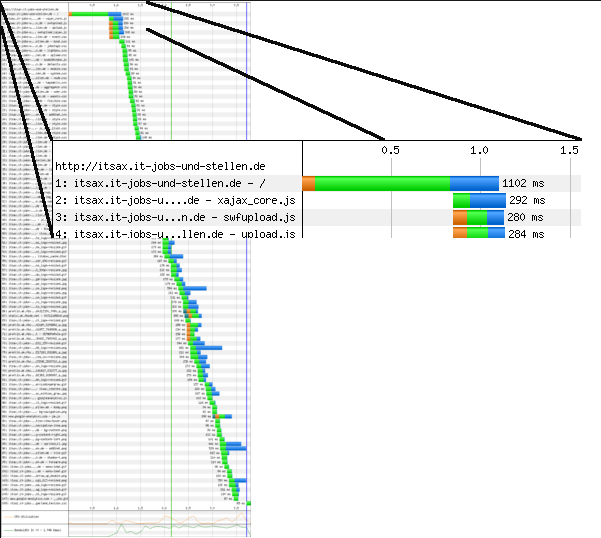
\includegraphics[scale=0.5]{material/start_waterfall_edited.png}
  \caption{Wasserfalldiagramm: Ausgangszustand}
  \label{fig:startwaterfall}
\end{figure}

%Load Time: 3.728
%Time to First Byte: 0.674s 	
%Time to Start Render: 2.002s
%\#DOM Elements: 855 	

%TODO TABELLE!



\begin{lstlisting}[language=bash,label=Ausgabe von ab,caption=Ausgabe von ab]
Server Software:        Apache/2.2.16
Server Hostname:        itsax.it-jobs-und-stellen.deDocument Path:          /
Document Length:        65218 bytes

Concurrency Level:      1
Time taken for tests:   18.182 seconds
Complete requests:      50

Write errors:           0
Total transferred:      3266726 bytes
HTML transferred:       3239226 bytes
Requests per second:    2.75 [#/sec] (mean)
Time per request:       363.640 [ms] (mean)
Time per request:       363.640 [ms] (mean, across all concurrent requests)
Transfer rate:          175.46 [kBytes/sec] received
\end{lstlisting}

\section{Implementierung und Test der einzelnen Methoden}
Im folgenden Abschnitt werden die eingesetzten Methoden dargestellt und ihre Auswirkungen auf die Webperformance der Seite ITsax.de aufgezeigt. 
Dabei werden alle Methoden, die vom Autor, nach der Analyse des Ausgangszustands, für möglicherweise sinnvoll befunden wurden, getestet. Die Methode wird jeweils mit dem Startwert verglichen und der Aufwand eingeschätzt.
\subsection{Alternative PHP Cache} Als allererste Maßnahme wurde ein PHP-Opcode-Cache untersucht. Opcode-Caches speichern das Kompilat vorangegangener Operationen und können so beim nächsten Aufruf direkt die Berechnung ausf\"uhren. Solche Systeme sind immer zu empfehlen, da sie normalerweise keinerlei Probleme bereiten und alle PHP Anfragen beschleunigen. Aktuell gibt es mehrere dieser, auch PHP-Beschleuniger genannte, Opcode-Caches. Unter ihnen nimmt aber der Alternative PHP Cache(APC)\footnote{\url{http://pecl.php.net/package/APC}} eine führende Position ein. Hauptsächlich weil es der zuverlässigste unter den nicht-kommerziellen Caches ist. Ab PHP Version 5.4 wird er in PHP schon enthalten sein.
%Quelle
Die Installation von APC ist auf einigermaßen aktuellen Linux Servern auch denkbar einfach. Das PHP-Pear-Framework, was oft schon installiert ist, erlaubt mit einigen wenigen Befehlen einen funktionierenden Opcode-Cache zu installieren. 
\begin{lstlisting}[language=bash,label=Installation von APC,caption=Installation von APC]
apt-get install php-pear
pecl install apc
\end{lstlisting}
Nach der Installation wurde die Antwortzeit des Apacheservers gemessen und es kam zu folgendem Ergebnis. Statt 363 ms wurden nur noch 233 ms benötigt. Das bedeutet eine Verbesserung um 36\% und es können 4,28 Anfragen je Sekunde bearbeitet werden gegenüber vorher nur 2,75. Alles unter der Prämisse, dass es keine nebnl\"aufigen Anfragen gibt. 
\begin{lstlisting}[language=bash,label=Ausgabe von ab,caption=Ausgabe von ab]
Server Software:        Apache/2.2.16
Server Hostname:        itsax.it-jobs-und-stellen.de
Server Port:            80

Document Path:          /
Document Length:        64842 bytes

Concurrency Level:      1
Time taken for tests:   11.681 seconds
Complete requests:      50

Write errors:           0
Total transferred:      3261730 bytes
HTML transferred:       3234230 bytes
Requests per second:    4.28 [\#/sec] (mean)
Time per request:       233.620 [ms] (mean)
Time per request:       233.620 [ms] (mean, across all concurrent requests)
Transfer rate:          272.69 [kBytes/sec] received
\end{lstlisting}
\subsection{Drupal Cache}Der Drupal Cache wurde mit Version 5 eingef\"uhrt und kann \"uber das Administrationsinterface aktiviert werden. Durch ihn wird ein Caching aller Seiten ausgel\"o\ss{}t. Dabei werden die fertig berechneten Webseiten beim ersten Aufruf komplett in der Datenbank abgelegt. Wenn eine schon gecachte Seite aufgerufen wird muss nur noch der fertige HTML-Code aus der Datenbank geh\"olt werden. Diese Methode ist aber zu unflexibel, da nicht konfigurierbar ist welche Seiten gecacht werden sollen. F\"ur die Webseite ITsax.de m\"ussen aber dynamische Inhalte ungecacht bleiben. Testweise wurde der Cache aktiviert und mit "`ab"' getestet. Die Erbnisse sind in folgender Ausgabe zu sehen. Die Zeit pro Anfrage wird deutlich kleiner und es wird klar dass Caching f\"ur den serverseitigen Teil die gr\"o\ss{}ten Verbesserungen bringt. Die PHP-Codeausführung kann auf ein notwendiges Minimum, dass heisst auf die Momente in denen der Cache neu geschrieben wird, reduziert werden. So kann zumindest der zu berechnende HTML-Code direkt ausgeliefert werden.
\begin{lstlisting}[language=bash,label=Ausgabe von ab,caption=Ausgabe von ab]
Server Software:        Apache/2.2.16
Server Hostname:        itsax.it-jobs-und-stellen.de
Server Port:            80

Document Path:          /
Document Length:        65005 bytes

Concurrency Level:      1
Time taken for tests:   2.082 seconds
Complete requests:      50
Failed requests:        0
Write errors:           0
Total transferred:      3276900 bytes
HTML transferred:       3250250 bytes
Requests per second:    24.02 [\#/sec] (mean)
Time per request:       41.638 [ms] (mean)
Time per request:       41.638 [ms] (mean, across all concurrent requests)
Transfer rate:          1537.09 [kBytes/sec] received
\end{lstlisting}

\subsection{JS Aggregation und Minifizierung mit dem Javascript Aggregation Modul}
Aggregation und Minifizierung sind Verfahren, die in der Web-Performance-Optimierung häufig eingesetzt werden. Für das Drupal 5 System gibt es fertige Module, die diese Aufgabe übernehmen. Das Modul interveniert innerhalb des Drupal Kerns. Dort werden die Javascripte ersetzt, die vorher direkt so ausgegeben wurden wie sie die Module lieferten. Stattdessen wird eine einzelne, das heisst aggregierte Version, die optional minifiziert werden kann, ausgeliefert. Diese Minifizierung wird natürlich genutzt und spart einige kB. Minifizierung wird ermöglicht durch die Nutzung von JSmin\footnote{Bibliothek zur Minifizierung von JavaScript. \url{https://github.com/rgrove/jsmin-php/}}. JSmin ist ein Filter, der unter anderem Kommentare entfernt und mehrere Leerzeichen zu einem zusammenfasst. Durch die Nutzung dieser Methode konnten 11 HTTP Abfragen und 11 kB an Datenvolumen eingespart werden.
%Load Time: 3.658s
%Time to First Byte: 0.595s
%Time to Start Render: 1.915s
%\#DOM Elements: 844 	
%\#Requests: 95 %!
%Bytes In: 432 kB
%http://www.webpagetest.org/result/110809_Z1_198TK/

\subsection{CSS Aggregation und Komprimierung}
Analog zur Javascript Optimierung kann man auch die CSS Aggregation betrachten. Dabei werden durch Zusammenfassung der einzelnen CSS Dateien HTTP Abfragen eingespart. Wie man an der gesunkenen Anzahl der Requests sehen kann, wurden 21 Abfragen nur durch Zusammenfügen der einzelnen CSS Dateien zu einer einzigen eingespart. Durch die Bereinigung beziehungsweise Komprimierung werden dabei außerdem 17 kB an überflüssigen Zeichen entfernt. 
%Load Time: 3.577s
%Time to First Byte: 0.649s
%Time to Start Render: 1.577s
%\#DOM Elements: 834 	
%\#Requests: 85 %!
%Bytes In: 427 kB
%http://www.webpagetest.org/result/110809_XB_198VE/
\subsection{Drupal Boost Modul} Das Boost Modul ist ein Cache für statische Seiten, der allerdings nur für nicht-angemeldete Gastnutzer funktioniert. Da ITsax.de fast ausschließlich von Gastnutzern besucht wird, bietet es sich an, dieses Modul zum Cachen kompletter Seiten zu nutzen. Dabei k\"onnen HTML, XML, Ajax, CSS und Javascript Dokumente gecacht werden. Zus\"atzlich k\"onnen diese durch gzipping\footnote{?} komprimiert werden.
%TODO footnote
Die genutzen Techniken sind sehr performant und bauen auf einem Dateisystemcache auf. Das bedeutet, jede Seite wird komplett auf der Festplatte abgelegt. Alle Arten von serverseitigen Prozessen werden so nach dem initialem Seitenaufruf, der das Caching auslöst, nicht mehr durchlaufen. Dies sieht man sehr gut an der Time to First Byte. Von den 172 ms werden ca. 50ms für den DNS Lookup benötigt und 70ms für die erste HTTP Verbindung. Der Server braucht demnach nur ca. 50 ms um die Seite auszuliefern. Dies hat natürlich einen sehr positiven Einfluss auf die Gesamtperformance und macht sich besonders beim Endnutzer bemerkbar, da die Seite spürbar schneller anfängt, sich im Browser aufzubauen. 
%Load Time: 3.233s
%Time to First Byte: 0.172s %!
%Time to Start Render: 1.473s
%\#DOM Elements: 856 	
%\#Requests: 106 %!
%Bytes In: 444 kB
%http://www.webpagetest.org/result/110809_AP_198XJ/

\subsection{Bildkompression mit jpegoptim und OptiPNG}
Bilder und Grafiken bieten oft großen Optimierungsspielraum. Zum einen erfolgt dies durch die richtige Auswahl der Dateiformate und zum anderen durch Komprimierung der Bilder. Da es auf www.itsax.de nicht nur statische Inhalte gibt, sondern auch durch Communitymitglieder und Communitymanager eingestellte Inhalte verwaltet werden müssen, sollte eine nachträgliche Qualitätsoptimierung der hochgeladenen Bilder durchgeführt werden. Um dies umzusetzen, sind die Programme OptiPNG und jpegOptim zu empfehlen. Da es sich bei beiden Programmen um Kommandozeilenprogramme handelt, kann man ihre Anwendung leicht automatisieren. Mit dem Linuxbefehl find, der praktischerweise eine Möglichkeit, Befehle auszuführen, besitzt, kann man direkt die entsprechenden Dateien an die Optimierer übergeben. Diese Aktionen können dann über einen Cronjob periodisch jede Nacht ausgeführt werden. 

\subsubsection{Verlustfreie Kompression} Technisch wird eine verlustfreie Kompression durch Verfahren wie die Huffman-Codierung oder die Lauflängenkodierung umgesetzt. Im Fall des PNG Formats wird die Komprimierungsmethode Deflate genutzt. Außerdem werden Vorfilter, in Form von prädikativer Kodierung, eingesetzt. Diese berechnen die wahrscheinlichen Farbwerte und es müssen nur die Abweichungen gespeichert werden. 
%TODO quelle

Die Befehle sehen dann wie folgt aus:

\begin{lstlisting}[language=bash,label=Optimieren mit find,caption=Optimieren mit find]
find . -name "*.png" -exec optipng -o7 {} \;
find . -name "*.jpg" -exec jpegoptim {} \;
\end{lstlisting}
Auf jeden Fall sollte eine verlustfreie Komprimierung durchgeführt werden, da die Bilder in diesem Fall nur an Dateigröße verlieren und die Bildqualität unberührt bleibt. 
%%http://optipng.sourceforge.net/
%%http://www.kokkonen.net/tjko/projects.html
%Load Time: 3.640
%Time to First Byte: 0.636s %!
%Time to Start Render: 1.894s
%\#DOM Elements: 855 	
%\#Requests: 106 %!
%Bytes In: 429 kB % 15kb gespart
%http://www.webpagetest.org/result/110809_C4_1999C/
\subsubsection{Verlustbehaftete Kompression} Da im Web kein besonders hoher Detailgrad gewährleistet werden muss, ist auch eine Kompression erwünscht, die auf Kosten der Bildqualität die Bildgröße verringert. 
\begin{lstlisting}[language=bash,label=Optimieren mit find,caption=Optimieren mit find]
find . -name "*.png" -exec optipng -o7 {} \;
find . -name "*.jpg" -exec jpegoptim {} \;
\end{lstlisting}
Load Time: 3.255s
Time to First Byte: 0.669s %!
Time to Start Render: 1.908s
\#DOM Elements: 855 	
\#Requests: 106 %!
Bytes In: 371 kB % 73kb gespart
%http://www.webpagetest.org/result/110809_15_199GY/

\subsection{Drupal 5 Fehler bei umgefärbten Themes}
Das Framework Drupal 5 benutzt Themes zur Gestaltung der Oberfläche. Um diese farblich anpassen zu können, wurde das Color Modul installiert, welches Themeveränderungen ermöglicht. Aufgrund der Tatsache, dass das Theme nur kopiert wird und im Anschluss die Farben geändert werden, entstehen bei diesem Vorgang unnötige Duplikate, die beim Laden der Seite mitgeschleppt werden. Um diese zu entfernen, wird einfach das Standardtheme durch das Modifizierte ersetzt. Dafür müssen  nur noch einige Pfade in der style.css angepasst werden und man spart in dem Fall von itsax.de 4 kB, was immerhin ca 1\% der übertragenen Datenmenge ausmacht. Umgesetzt wurde diese Ma\ss{}nahme, indem die Duplikate manuell zu einer Datei zusammengef\"uhrt wurden. Oftmals m\"ussen nur Farbangaben ersetzt werden um die gew\"unschten resulatete zu erzielen. Danach wird das Theme durch das Zusammengef\"uhrte ersetzt. Das Color Modul kann dann deaktiviert werden.
%Load Time: 3.626s
%Time to First Byte: 0.629s %!
%Time to Start Render: 1.890s
%\#DOM Elements: 854 	
%\#Requests: 104 %!
%Bytes In: 440 kB % 4kb gespart
%http://www.webpagetest.org/result/110809_SZ_19APH/

\subsection{Theme Bilder spriten}
Spriting wurde ursprünglich in der Videospielentwicklung verwendet, um Bilder in den Grafikspeicher zu laden. In der Webentwicklung ist es eine effektive Technik, um Bilder ohne mehrfachen Overhead zu laden. Beim Spriting wird aus vielen Einzelbildern eine Gesamtgrafik erstellt. Um auf die Ursprungsbilder dann einzeln zugreifen zu können, werden CSS Befehle genutzt, die es ermöglichen, die Größe und die Position eines Bildausschnittes anzuzeigen. 
%Load Time: 3.707
%Time to First Byte: 0.669s %!
%Time to Start Render: 1.968s
%\#DOM Elements: 855 	
%\#Requests: 103 
%Bytes In: 443 kB 
%http://www.webpagetest.org/result/110810_FZ_19GBA/

\subsection{Module von Startseite entfernen}
Um zu überprüfen, welchen Einfluss verschiedene, im Netzwerkgraphen auffällige, Module auf die Gesamtperformance haben, werden sie testweise komplett deaktiviert. So kann man entscheiden, bei welchen Modulen zusätzlicher Programmieraufwand lohnenswert ist.
\subsubsection{Partnerslideshow} Das Deaktivieren der Partnerslideshow hat gravierenden Einfluss auf die Gesamtperformance. Das Modul lädt im aktiven Zustand alle Bilder, die es benötigt und bremst damit den gesamten Ladevorgang aus. Die Ladezeit verringert sich um 27,7\%. Der größte Teil des Geschwindigkeitszuwachses ist der Verringerung der Übertragungsmenge zuzuschreiben. 
%Load Time: 2.695s
%Time to First Byte: 0.636s %!
%Time to Start Render: 1.838s
%\#DOM Elements: 790
%\#Requests: 80
%Bytes In: 276 kB

\subsubsection{Facebook Widget} In diesem Fall ist der Einfluss auf die Performance geringer, aber mit einer Verbesserung von 6,7\% auf jeden Fall vorhanden. Das Widget besteht aus neun kleinen Fotos und dem Facebookrahmen. Den größten Effekt hat hier die Verringerung der Anzahl der HTTP Anfragen. So können wichtigere Elemente schneller geladen werden.
%Load Time: 3.478s
%ime to First Byte: 0.668s %!
%Time to Start Render: 1.966s
%\#DOM Elements: 779 	
%\#Requests: 95 
%Bytes In: 406 kB 

\subsubsection{Jobleiste deaktiviert} Die Jobleiste hat einen geringfügig größeren Einfluss auf die Ladezeiten als das Facebook Widget. Die Ursache ist wahrscheinlich in den zusätzlichen Bibliotheken zu suchen, die zu diesem Modul gehören. Darunter sind Ajax Bibliotheken und anderer ThirdParty Code. 
%Load Time: 3.367s
%Time to First Byte: 0.617s %!
%Time to Start Render: 1.709s
%\#DOM Elements: 822 	
%\#Requests: 94 
%Bytes In: 411 kB

\subsection{Umprogrammierung der Module}
Um die langsamen Module weiterhin nutzen zu können, muss eine Lösung gefunden werden, die es ermöglicht, Inhalte nachzuladen, nachdem die Seite komplett geladen wurde. Um diese Asynchronität zu erreichen, wird mit Hilfe eines Timeout-Befehls, das Laden der nicht priorisierten Inhalte verzögert. Programmiert wird dieses Verhalten mit Javascript, genauer JQuery. Besonders betrachtet werden muss dabei, ob eine vorhandene Dynamik erhalten bleiben soll. Dazu gehören zum Beispiel zufällige Elemente oder Elemente mit besonders häufigen Aktualisierungen.

\subsubsection{Partnerslideshow}
\begin{figure}[!ht]
  \centering
  
\includegraphics[scale=0.5]{material/partner_slideshow.png}
  \caption{Größe der Inhalte}
  \label{fig:startbyte}
\end{figure} Die Partnerslideshow ist eher ein kosmetisches Element der Startseite und für den Nutzer nicht notwendig. Daher kann es so programmiert werden, dass beim Laden nur ein leeres DIV übergeben wird. Dann wird ein Timeout gestartet und bei der Aktivierung des Timeoutevents wird das DIV mit den Slideshowelementen gefüllt sowie die Slideshow gestartet. Der Code wurde dahingehend angepasst, dass der HTML Code in eine Javascript Variable geschrieben wird, anstatt ihn direkt in der Seite einzufügen. Dadurch ist es möglich über eine DOM Manipulation den HTML Code später einzufügen. Das stellt sich dann wie im folgenden Codeaussschnitt dar.
\begin{lstlisting}[language=php,label=Javascript - Slideshow,caption=Javascript - Slideshow]
drupal_add_js('
  if (Drupal.jsEnabled) {
  $(document).ready(function() {
     window.setTimeout(delayed_partnerbox,500);
  });
  function delayed_partnerbox(){
	$("#projects").parent().html(partner_box_load);
	$(".slideshow").cycle({
	    delay:  200 ,
	    height: "80px",
	    width: "180px",
	    containerResize: 0,
	    fit: 1,
	    fx: "fade"
	});
  }
}', 'inline')
\end{lstlisting}
An das window Objekt wird in Zeile 3 ein Timer gehängt. Der Timer löst nach 500 ms einen Callback aus, durch den die Funktion delayed\_partnerbox ausgeführt wird. Durch diese Verlagerung des Inhalts braucht die Webseite nur noch 2.749s zum laden. Bis die Webseite die nachgeladene Slideshow anzeigt, vergehen 3.794s. Die Webseite ist also eher benutzbar und später komplett geladen. In Testverfahren, wie zum Beispiel für das Google Ranking wird nur betrachtet, wann die Seite das Onload Event auslöst. Somit wurde die Seite für Google und den Nutzer schneller. Der Performancegewinn geht wie in der vorherigen Analyse festgestellt aus der verringerten Datenmenge hervor. Natürlich spielt auch die Reduzierung der HTTP Anfragen eine Rolle. Die Datenmenge wurde auf 284 kB verringert und es wurden statt 107 nur 82 HTTP Anfragen benötigt.
%Time to First Byte: 0.626s %!
%Time to Start Render: 1.842s
%\#DOM Elements: 855 	
%\#Requests: 82 (107)
%Bytes In: 284 kB (395)
%http://www.webpagetest.org/result/110810_3Z_19MRE/

\subsubsection{Facebook Widget}
\begin{figure}[!ht]
  \centering
  
\includegraphics[scale=0.5]{material/facebook_widget.png}
  \caption{Größe der Inhalte}
  \label{fig:facebookwidget}
\end{figure} Das Modul für das Facebook Widget wurde durch Entwickler der pludoni GmbH so programmiert, dass es das von Facebook zur Verfügung gestellte Widget cacht und dann auf der Webseite darstellt. Das Hauptproblem bei dem Widget ist, dass die Profilbilder, die angezeigt werden, auf den Servern von Facebook liegen und sich somit der internen Kontrolle entziehen. Um das Modul abzukoppeln wird ein Timer analog zum vorhergehenden Modul programmiert. 
\begin{lstlisting}[language=php,label=Facebook Widget,caption=Facebook Widget]
function facebook_show_likebox() {
  $local_path = drupal_get_path("module","facebook_pludoni");
  drupal_add_js('
  if (Drupal.jsEnabled) {
      $(document).ready(function() {
      window.setTimeout(delayed_facebookbox,400);
    });
    function delayed_facebookbox(){
      $("#facebook-likebox").html("<iframe frameborder=\"0\" scrolling=\"no\" src=\"/'.$local_path.'/caching/likebox_cache.html\" id=\"fbooklikebox\"></iframe>");
    }
  }', 'inline');
  return '<div id="facebook-likebox"></div>';
}
\end{lstlisting}
Wieder wird als initialer Rückgabewert nur ein leeres DIV-Element ausgegeben. Diesmal kann der HTML Code aber direkt eingefügt werden, ohne den Umweg über eine Javascriptvariable gehen zu müssen. Durch die Verringerung der HTTP Anfragen um 11 und der Webseitengröße um 38 kB kann eine Verbesserung der Ladezeit von 300 ms erzielt werden. 
%Load Time: 3.411s (4.258)
%Time to First Byte: 0.576s %!
%Time to Start Render: 1.848s
%\#DOM Elements: 857
%\#Requests: 95 (106)
%Bytes In: 406 kB (444)
%http://www.webpagetest.org/result/110810_AJ_19N72/

\subsubsection{Partneranzeigen}
\begin{figure}[!ht]
  \centering
  
\includegraphics[width=1.1\textwidth]{material/partneranzeigen.png}
  \caption{Größe der Inhalte}
  \label{fig:partneranzeigen}
\end{figure}
Das Partneranzeigen-Modul musste umprogrammiert werden, da die Startseite durch das Boost Modul gecacht werden soll. Caching bedeutet normalerweise die Abwesenheit dynamischer oder zufälliger Elemente. Da aber bei jedem Besuch der Webseite ein zufälliger Communitypartner angezeigt werden soll, musste eine Lösung gefunden werden. Gelöst wurde das Problem durch Auslagerung des Codes in einen Callback, der unter einer anderen URI angesprochen werden kann. Das Boost Modul kann solche Inhalte auch cachen. Es ist aber auch über einen URI Filter konfigurierbar. So kann eine performante Startseite mit dynamischen Inhalten realisiert werden. Die Ladezeit wird durch diesen Umweg leider negativ beeinflusst, aber 100 ms stehen in keinem Verhältnis zu dem Gewinn, der später erzielt wird. Da in einer Drupal Umgebung gearbeitet wird, kann leicht über einen Menü hook dem System die neue URI mitgeteilt werden. Wenn sie, nachdem sie bekannt gemacht wurde, aufgerufen wird, liefert sie den einzufügenden HTML Code aus.
%TODO URI???
%menuhook???
\begin{lstlisting}[language=php,label=Ajax - hook,caption=Ajax - hook]
function partneranzeigen_menu() {
  $items = array();
  $items[] = array(
    'path'        => "partanz/ajax",
    'callback'    => 'partneranzeigen_display_block_1',
    'type'        => MENU_CALLBACK,
    'access'      => true
  );
  return $items;
}
\end{lstlisting}
Eingefügt wird der HTML Code dann über eine Ajax GET Anfrage. Mit der schon bekannten Timeout Methode.
\begin{lstlisting}[language=php,label=Ajax - GET,caption=Ajax - GET]
function delayed_partneranzeigen(){
  $.get('/partanz/ajax',function(data){
    $('#partneranzeigenbox').html(data);
});
\end{lstlisting}
Obwohl die Seite um 31 kB kleiner geworden ist und zwei HTTP Anfragen eingespart werden, wird sie, wie schon erwähnt, langsamer.
%Load Time: 3.871s (5.759s)
%Time to First Byte: 0.669s %!
%Time to Start Render: 2.255s
%\#DOM Elements: 857 
%\#Requests: 105 (108)
%Bytes In: 417 kB (448)
%http://www.webpagetest.org/result/110815_N6_1AWKT/1/details/


\section{Endergebnis} 
Nach der Zusammenführung aller Optimierungen wurde die Webseite erneut getestet. Das Wasserfalldiagramm der optimierten Webseite ist in Abbildung \ref{endwaterfall} dargestellt. 
\begin{figure}[!ht]
  \centering
  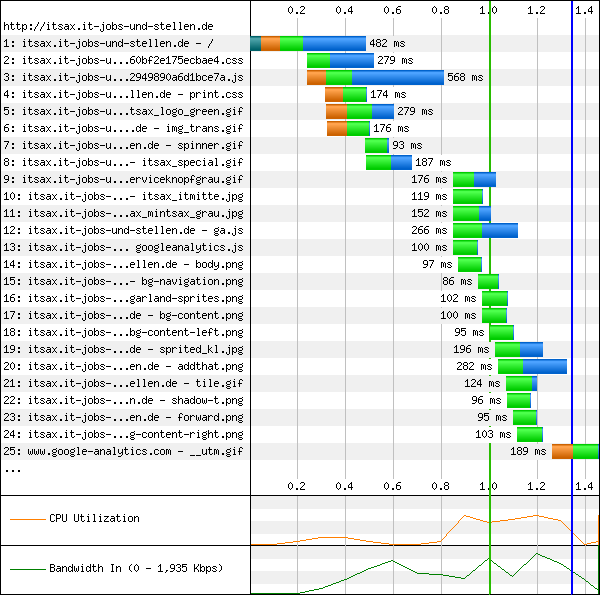
\includegraphics[scale=0.5]{material/end_waterfall.png}
  \caption{Wasserfalldiagramm: Optimierte Webseite}
  \label{fig:endwaterfall}
\end{figure}
Nach nur einer Sekunde fängt der Browser an die Seite darzustellen. 2,913 Sekunden werden benötigt bis alle asynchronen Inhalte verfügbar sind. Die Webseitengröße wurde auf 138 kB komprimiert. Daher können auch langsame Internetverbindungen die Seite schnell laden. Von den 107 HTTP Anfragen sind nur noch 67 übrig geblieben, von denen werden aber nur 25 vor dem Onload Event benötigt. Dank dieser Reduzierung auf das Wesentliche erwartet den Besucher nun eine subjektiv wesentlich angenehmere Webseite. 
\begin{figure}[!ht]
  \centering
  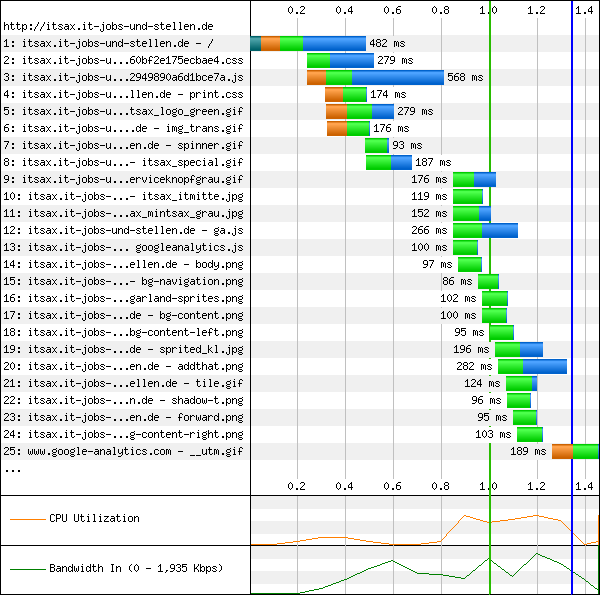
\includegraphics[scale=0.5]{material/end_waterfall.png}
  \caption{Wasserfalldiagramm: Optimierte Webseite}
  \label{fig:endwaterfall}
\end{figure}
%http://www.webpagetest.org/result/110825_5J_1DQHK/
\section{Vergleich}
Ein abschlie\ss{}ender Vergleich aller Methoden wurde tabellarisch zusammengetragen. In der ersten Spalte steht der Methodenname, darauf folgen die Gesamtladezeit und die Zeit die der Nutzer warten muss bis der Browser anf\"angt Inhalte darzustellen. Zu jedem Ergebnis wird noch ein kurzer Kommentar gegeben und in der letzten Zeile wurde das Gesamtergebnis eingetragen.
\begin{center}
    \begin{longtable}{ | p{3cm} | p{1.5cm} | p{1.5cm} | p{6cm} |}
    \hline
    Methode & Load Time & TtSR & Kommentar \\ \hline
    \hline
    Ausgangszustand 			& 3,728s (+0,00\%)  				& 2,002s (+0,00\%) & Der Ausgangszustand ohne Optimierungen. \\ \hline
    JS Aggregation 			& 3,658s \textcolor{green}{($-1,87\%$)}  	& 1,915s \textcolor{green}{($-4,35\%$)} & Bei geringen Aufwand können hier erste Verbesserungen erzielt werden. \\ \hline
    CSS Aggregation 			& 3,577s \textcolor{green}{($-4,05\%$)} 	& 1,577s \textcolor{green}{($-21,23\%$)}& Diese Optimierung sollte auch auf jeden Fall durchgeführt werden. \\ \hline
    Boost Modul 			& 3,233s \textcolor{green}{($-13,22\%$)} 	& 1,473s \textcolor{green}{($-26,42\%$)}& Caching ist Pflicht! Nur in seltenen Ausnahmen ist davon abzusehen. \\ \hline
    Bildkompression verlustfrei 	& 3,640s \textcolor{green}{($-2,31\%$)} 	& 1,894s \textcolor{green}{($-5,4\%$)}& Durch Verringerung der Datenmenge können besonders Handynutzer profitieren.  \\ \hline
    Bildkompression verlustbehaftet 	& 3,255s \textcolor{green}{($-12,68\%$)} 	& 1,908s \textcolor{green}{($-4,7\%$)}& Zusätzliche verlustbehaftete Kompression sorgt oft für schnelleren Seitenaufbau, da große Mengen an Daten eingespart werden können.  \\ \hline
    Drupal 5 Theme Fehler 		& 3,626s \textcolor{green}{($-2,73\%$)} 	& 1,890s \textcolor{green}{($-5,59\%$)}& Durch diese sehr spezielle Optimierung können auch 100ms gewonnen werden.  \\ \hline
    Theme Bilder gesprited 		& 3,707s \textcolor{green}{($-0,56\%$)} 	& 1,968s \textcolor{green}{($-1,69\%$)}& Spriting ist eine gute Möglichkeit Requests zu sparen, macht sich aber leider nicht stark in der Ladezeit bemerkbar.  \\ \hline
    Partnerslideshow 			& 2,749s \textcolor{green}{($-26,26\%$)}  	& 1,842s \textcolor{green}{($-7,99\%$)}& Sehr deutlich wird die Geschwindigkeit durch das asynchrone Nachladen von Inhalten verbessern.  \\ \hline
    Facebook Widget 			& 3,411s \textcolor{green}{($-8,50\%$)} 	& 1,848s \textcolor{green}{($-7,69\%$)}& Besonders bei Inhalten von externen Quellen ist es nützlich die Ladezeiten abzukoppeln.  \\ \hline
    Partneranzeigen 			& 3,871s \textcolor{red}{(+3,83\%)} 		& 2,225s \textcolor{red}{(+11.13\%)}& An diesem Beispiel wird deutlich, dass nachladen nicht unbedingt Verbesserung sein muss. Trotzdem ist diese Umprogrammierung nötig, um das Caching der Startseite zu ermöglichen.  \\ \hline
    \hline 
    \hline
    Gesamtergebnis 			& 1.354s \textcolor{green}{($-63,68\%$)} & 0.952s \textcolor{green}{($-52,45\%$)} & Wenn alle Verbesserungen auf einmal aktiviert werden, wird die Webseite dramatisch beschleunigt.  \\ \hline
    
    \hline
    \end{longtable}
\end{center}


\section{Zusammenfassung und Ausblick}
Im Rahmen dieser Arbeit wurde beispielhaft an der Startseite der Community ITsax eine Web-Performanceanalyse durchgef\"uhrt und offensichtliche Fehler behoben. Zus\"atzlich wurden die Verbesserungen so dokumentiert, dass sie auf alle anderen Portale der pludoni GmbH leicht angewendet werden k\"onnen. Auf dem Gebiet der Web-Performance gibt es st\"andig neue Entwicklungen, da sehr viele exzellente Programmierer in Firmen wie Google, Microsoft und Yahoo an dieser Entwicklung beteiligt wird. Oftmals ist es daher schwer die effektivsten Verbesserungen heraus zu Filtern und Priorit\"aten zu setzen. Die Arbeit hat gezeigt das ein Fokus auf die Bereiche HTTP-Anfragen und Webseitengr\"o\ss{}e verringern schon zu sehr guten Ergebnissen f\"uhrt. Weiterf\"uhrende Ma\ss{}nahmen k\"onnten zum Beispiel die Nutzung von CDN Services sein. Auch ein aktuellere Drupal Version k\"onnte in Betracht gezogen werden, dies ist aber mit einem erheblichen Zeitaufwand verbunden. 
Da der Fokus dieser Arbeit nur auf der Startseite lag wurden andere kritische Bereiche wie zum Beispiel die Suche noch nicht betrachtet. Gerade bei dynamischen Elementen wie der Suche w\"are eine weiterf\"uhrende Besch\"aftigung mit den M\"oglichkeiten Profiling und Debugging bieten anzuraten.


